\begin{flushright} {\tiny {\color{gray} basis\_Q28\_2D.tex}} \end{flushright}
%~~~~~~~~~~~~~~~~~~~~~~~~~~~~~~~~~~~~~~~~~~~~~~~~~~~~~~~~~~~~~~~~~~~~~~~~~~~~~~~~~~~~~~~~~~~~~~~~~~

The serendipity elements are those rectangular elements which have no
interior nodes (See for example Reddy \cite[p65]{reddybook2}).
Inside an element a possible local numbering of the nodes is as follows:

\begin{flushright} {\tiny {\color{gray} (tikz\_serendipity2d.tex)}} \end{flushright}
%~~~~~~~~~~~~~~~~~~~~~~~~~~~~~~~~~~~~~~~~~~~~~~~~~~~~~~~~~~~~~~~~~~~~~~~~~~~~~~~~~~~~~~~~~~~~~~~~~~

\begin{center}
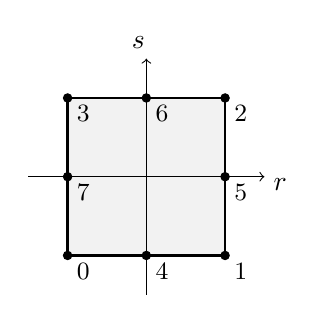
\begin{tikzpicture}
%\draw[step=0.5cm,gray,very thin] (0,0) grid (4,4); 
\draw[fill=gray!10,gray!10](1,1) rectangle (3,3);
\draw[thick] (1,1)--(3,1)--(3,3)--(1,3)--cycle;
\draw [->] (0.5,2) -- (3.5,2);
\draw [->] (2,0.5) -- (2,3.5);
\node[] at (3.7,1.9) {$r$};
\node[] at (1.9,3.7) {$s$};
\draw[black,fill=black] (1,1)   circle (1.5pt);
\draw[black,fill=black] (1,2)   circle (1.5pt);
\draw[black,fill=black] (1,3)   circle (1.5pt);
\draw[black,fill=black] (2,1)   circle (1.5pt);
\draw[black,fill=black] (2,3)   circle (1.5pt);
\draw[black,fill=black] (3,1)   circle (1.5pt);
\draw[black,fill=black] (3,2)   circle (1.5pt);
\draw[black,fill=black] (3,3)   circle (1.5pt);
\node[] at (1.2,0.8) {\small $0$};
\node[] at (2.2,0.8) {\small $4$};
\node[] at (3.2,0.8) {\small $1$};
\node[] at (1.2,1.8) {\small $7$};
\node[] at (3.2,1.8) {\small $5$};
\node[] at (1.2,2.8) {\small $3$};
\node[] at (2.2,2.8) {\small $6$};
\node[] at (3.2,2.8) {\small $2$};
\end{tikzpicture}
\end{center}


The main difference with the $Q_2$ element resides in the fact that there is 
no node in the middle of the element.
The polynomial representation of the function $\phi$ over the element is then
\[
\phi_h(r,s) = a + br + cs + drs + er^2 + fs^2 + gr^2s + hrs^2
\]
Note that absence of the $r^2s^2$ term which was previously associated 
to the center node. We find that 
\begin{mdframed}[backgroundcolor=blue!5]
\begin{eqnarray}
\bN_0(r,s)&=& \frac{1}{4}(1-r)(1-s)(-r-s-1) \\
\bN_1(r,s)&=& \frac{1}{4}(1+r)(1-s)(r-s-1) \\
\bN_2(r,s)&=& \frac{1}{4}(1+r)(1+s)(r+s-1) \\
\bN_3(r,s)&=& \frac{1}{4}(1-r)(1+s)(-r+s-1) \\
\bN_4(r,s)&=& \frac{1}{2}(1-r^2)(1-s)  \\
\bN_5(r,s)&=& \frac{1}{2}(1+r)  (1-s^2)\\
\bN_6(r,s)&=& \frac{1}{2}(1-r^2)(1+s)  \\
\bN_7(r,s)&=& \frac{1}{2}(1-r)  (1-s^2)
\end{eqnarray}
\end{mdframed}

The basis functions at the mid side nodes are products of a 
second order polynomial parallel to side and 
a linear function perpendicular to the side
while basis functions for corner nodes are modifications of the bilinear
quadrilateral element.

\begin{center}
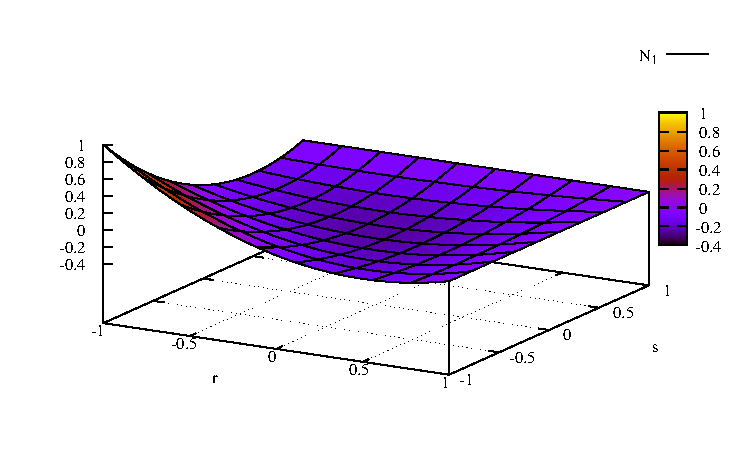
\includegraphics[width=4cm]{images/basis_Q28_2D/N1}
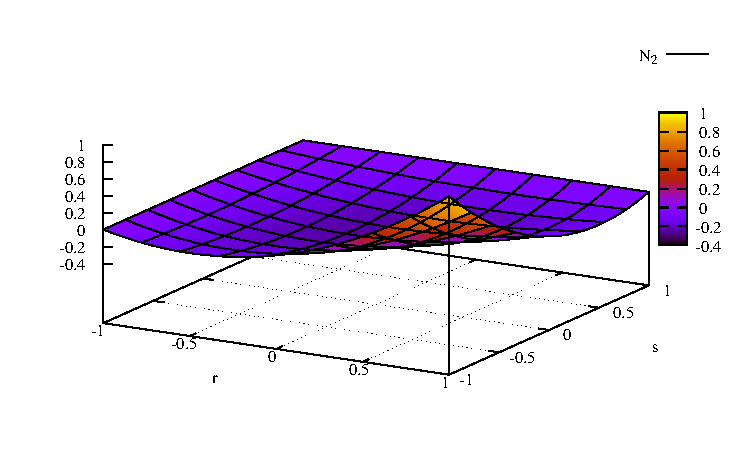
\includegraphics[width=4cm]{images/basis_Q28_2D/N2}
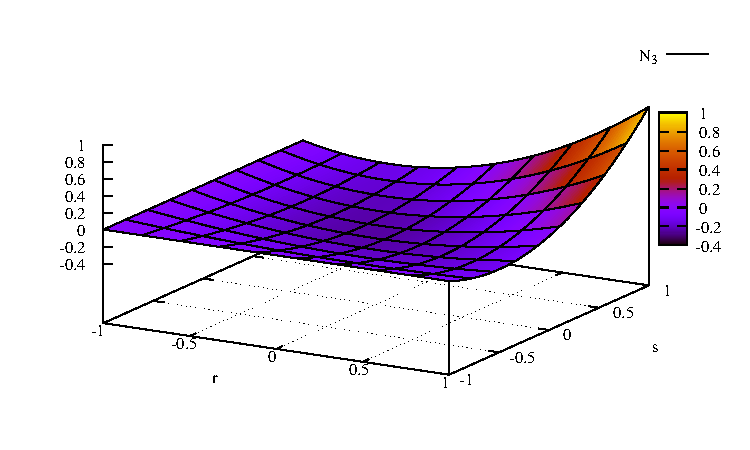
\includegraphics[width=4cm]{images/basis_Q28_2D/N3}
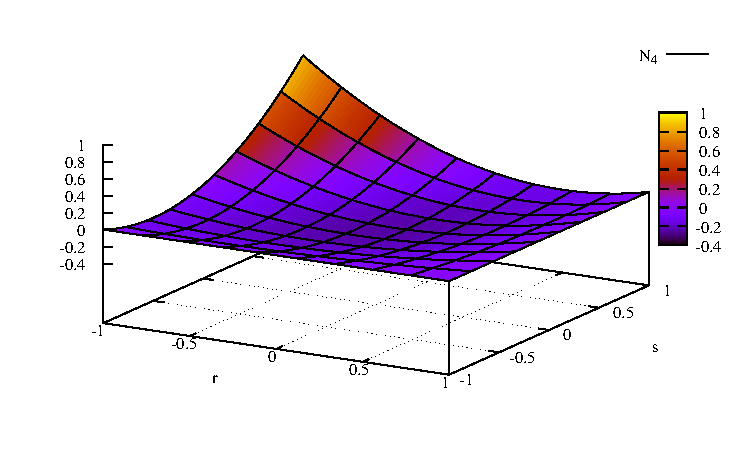
\includegraphics[width=4cm]{images/basis_Q28_2D/N4}\\
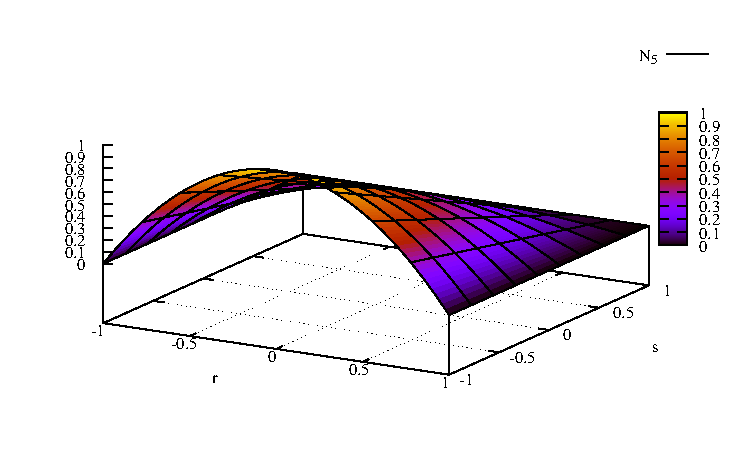
\includegraphics[width=4cm]{images/basis_Q28_2D/N5}
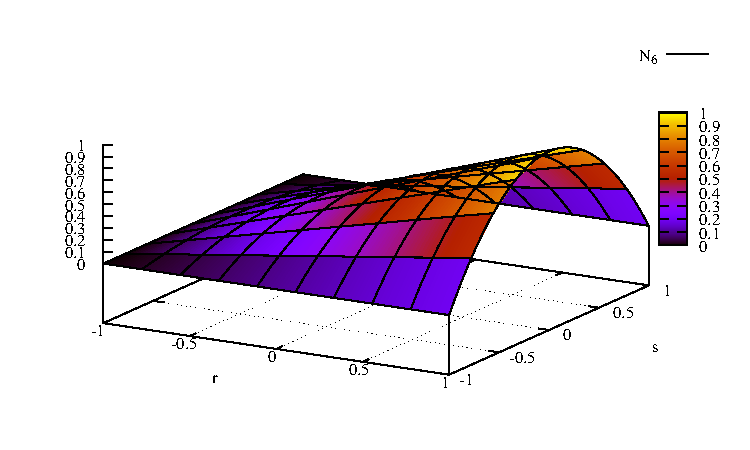
\includegraphics[width=4cm]{images/basis_Q28_2D/N6}
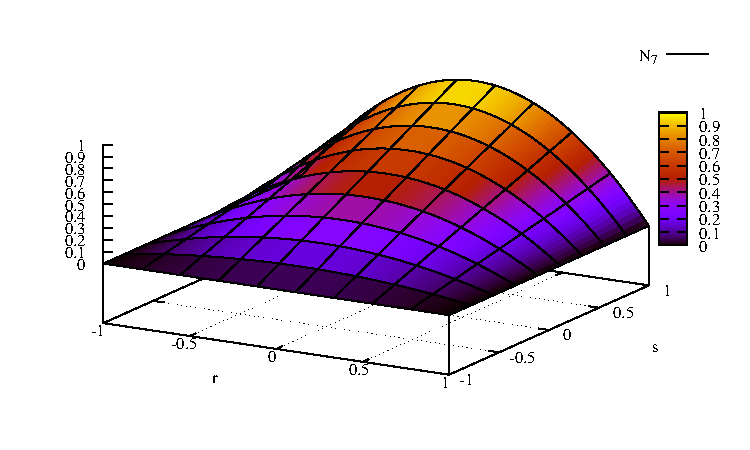
\includegraphics[width=4cm]{images/basis_Q28_2D/N7}
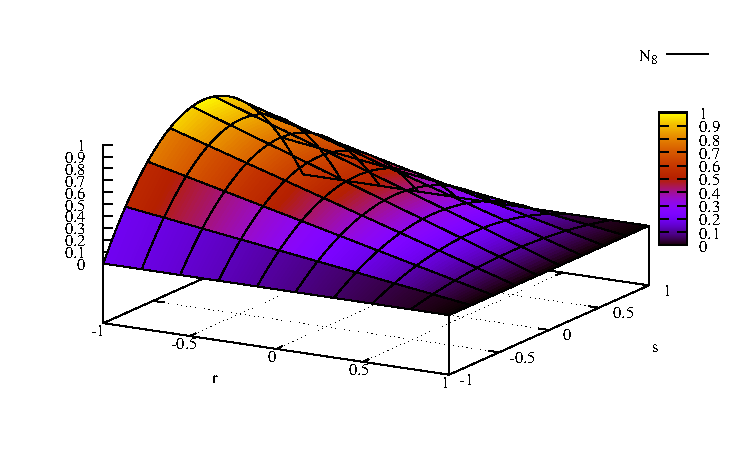
\includegraphics[width=4cm]{images/basis_Q28_2D/N8}\\
{\captionfont Surface representation of the basis functions on the reference element.
{\color{gray} in images/basis\_Q28\_2D/ }}
\end{center}



The first-order derivatives are given by:

\begin{mdframed}[backgroundcolor=blue!5]
\begin{eqnarray}
\frac{\partial \bN_0}{\partial r}(r,s)&=& -\frac{1}{4}(s-1)(2r+s)  \\
\frac{\partial \bN_1}{\partial r}(r,s)&=& -\frac{1}{4}(s-1)(2r-s)  \\
\frac{\partial \bN_2}{\partial r}(r,s)&=& \frac{1}{4}(s+1)(2r+s)  \\
\frac{\partial \bN_3}{\partial r}(r,s)&=& \frac{1}{4}(s+1)(2r-s)  \\
\frac{\partial \bN_4}{\partial r}(r,s)&=& r(s-1)  \\
\frac{\partial \bN_5}{\partial r}(r,s)&=& \frac{1}{2} (1-s^2)  \\
\frac{\partial \bN_6}{\partial r}(r,s)&=& -r(s+1)  \\
\frac{\partial \bN_7}{\partial r}(r,s)&=& -\frac{1}{2} (1-s^2)  
\end{eqnarray}
\end{mdframed}

\begin{mdframed}[backgroundcolor=blue!5]
\begin{eqnarray}
\frac{\partial \bN_0}{\partial s}(r,s)&=& -\frac{1}{4}(r-1)(r+2s) \\
\frac{\partial \bN_1}{\partial s}(r,s)&=& -\frac{1}{4}(r+1)(r-2s) \\
\frac{\partial \bN_2}{\partial s}(r,s)&=&  \frac{1}{4}(r+1)(r+2s) \\
\frac{\partial \bN_3}{\partial s}(r,s)&=&  \frac{1}{4}(r-1)(r-2s) \\
\frac{\partial \bN_4}{\partial s}(r,s)&=& - \frac{1}{2}(1-r^2)\\
\frac{\partial \bN_5}{\partial s}(r,s)&=&  -(r+1)s \\
\frac{\partial \bN_6}{\partial s}(r,s)&=& \frac{1}{2} (1-r^2)\\
\frac{\partial \bN_7}{\partial s}(r,s)&=&  (r-1)s
\end{eqnarray}
\end{mdframed}
These basis functions are used in \stone 52.
